\documentclass[tikz,border=10pt]{standalone}
\usepackage{tikz}
\usetikzlibrary{calc, intersections} % 修正拼写错误：intersecctons → intersections

\begin{document}
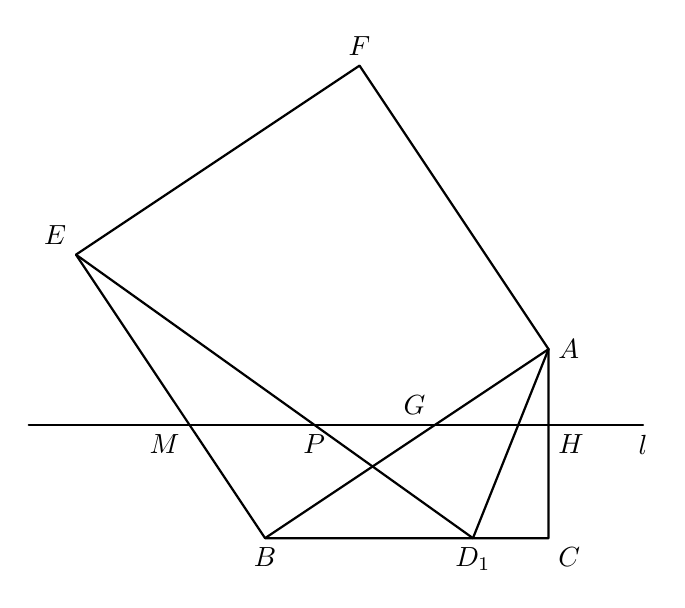
\begin{tikzpicture}[line cap=round, line join=round, >=stealth, scale=1.2]

    % --- 1. 定义核心顶点坐标 ---
    % 以 C 点为原点 (0,0)
    \coordinate (C) at (0,0);
    \coordinate (B) at (-3,0);
    \coordinate (A) at (0,2);
    
    % 计算正方形 ABEF 的顶点 (假设正方形在向量 AB 的左侧)
    % 向量 AB = B - A = (-3, -2)
    % 垂直向量为 (2, -3) 或 (-2, 3)
    \coordinate (E) at ($(B) + (-2, 3)$);
    \coordinate (F) at ($(A) + (-2, 3)$);

    % --- 2. 定义水平参考线 l ---
    % 穿过 G, H 的水平线，高度约为 A 点下方 0.8 单位
    \coordinate (L_left) at (-5.5, 1.2);
    \coordinate (L_right) at (1, 1.2);
    % 关键修改：移除 dash pattern=on 2pt off 2pt，改为实线
    \draw[thick] (L_left) -- (L_right) node[below] {$l$};

    % --- 3. 计算交点 ---
    % 直线 AB 与水平线 l 的交点 G
    \coordinate (G) at (intersection of B--A and L_left--L_right);
    % 直线 AC 与水平线 l 的交点 H (此处 AC 是垂直线)
    \coordinate (H) at (0, 1.2);
    % 直线 BE 与水平线 l 的交点 M
    \coordinate (M) at (intersection of B--E and L_left--L_right);
    
    % 特殊点 D1 在 BC 上
    \coordinate (D1) at (-0.8, 0);
    
    % 直线 ED1 与水平线 l 的交点 P
    \coordinate (P) at (intersection of E--D1 and L_left--L_right);

    % --- 4. 绘制实线几何轮廓 ---
    \draw[thick] (A) -- (B) -- (C) -- cycle; % 直角三角形 ABC
    \draw[thick] (B) -- (E) -- (F) -- (A);   % 正方形/四边形边框
    
    % --- 5. 绘制辅助虚线 ---
    \draw[thick] (E) -- (D1);
    \draw[thick] (A) -- (D1);

    % --- 6. 标注点名称 ---
    \node[right] at (A) {$A$};
    \node[below] at (B) {$B$};
    \node[below right] at (C) {$C$};
    \node[above left] at (E) {$E$};
    \node[above] at (F) {$F$};
    \node[above left] at (G) {$G$};
    \node[below right] at (H) {$H$};
    \node[below left] at (M) {$M$};
    \node[below] at (P) {$P$};
    \node[below] at (D1) {$D_1$};

\end{tikzpicture}
\end{document}